\section{Patch Collection Process}
\begin{frame}
  \frametitle{Patch Collection}
  \framesubtitle{First Area of Complexity}
  \begin{figure}
    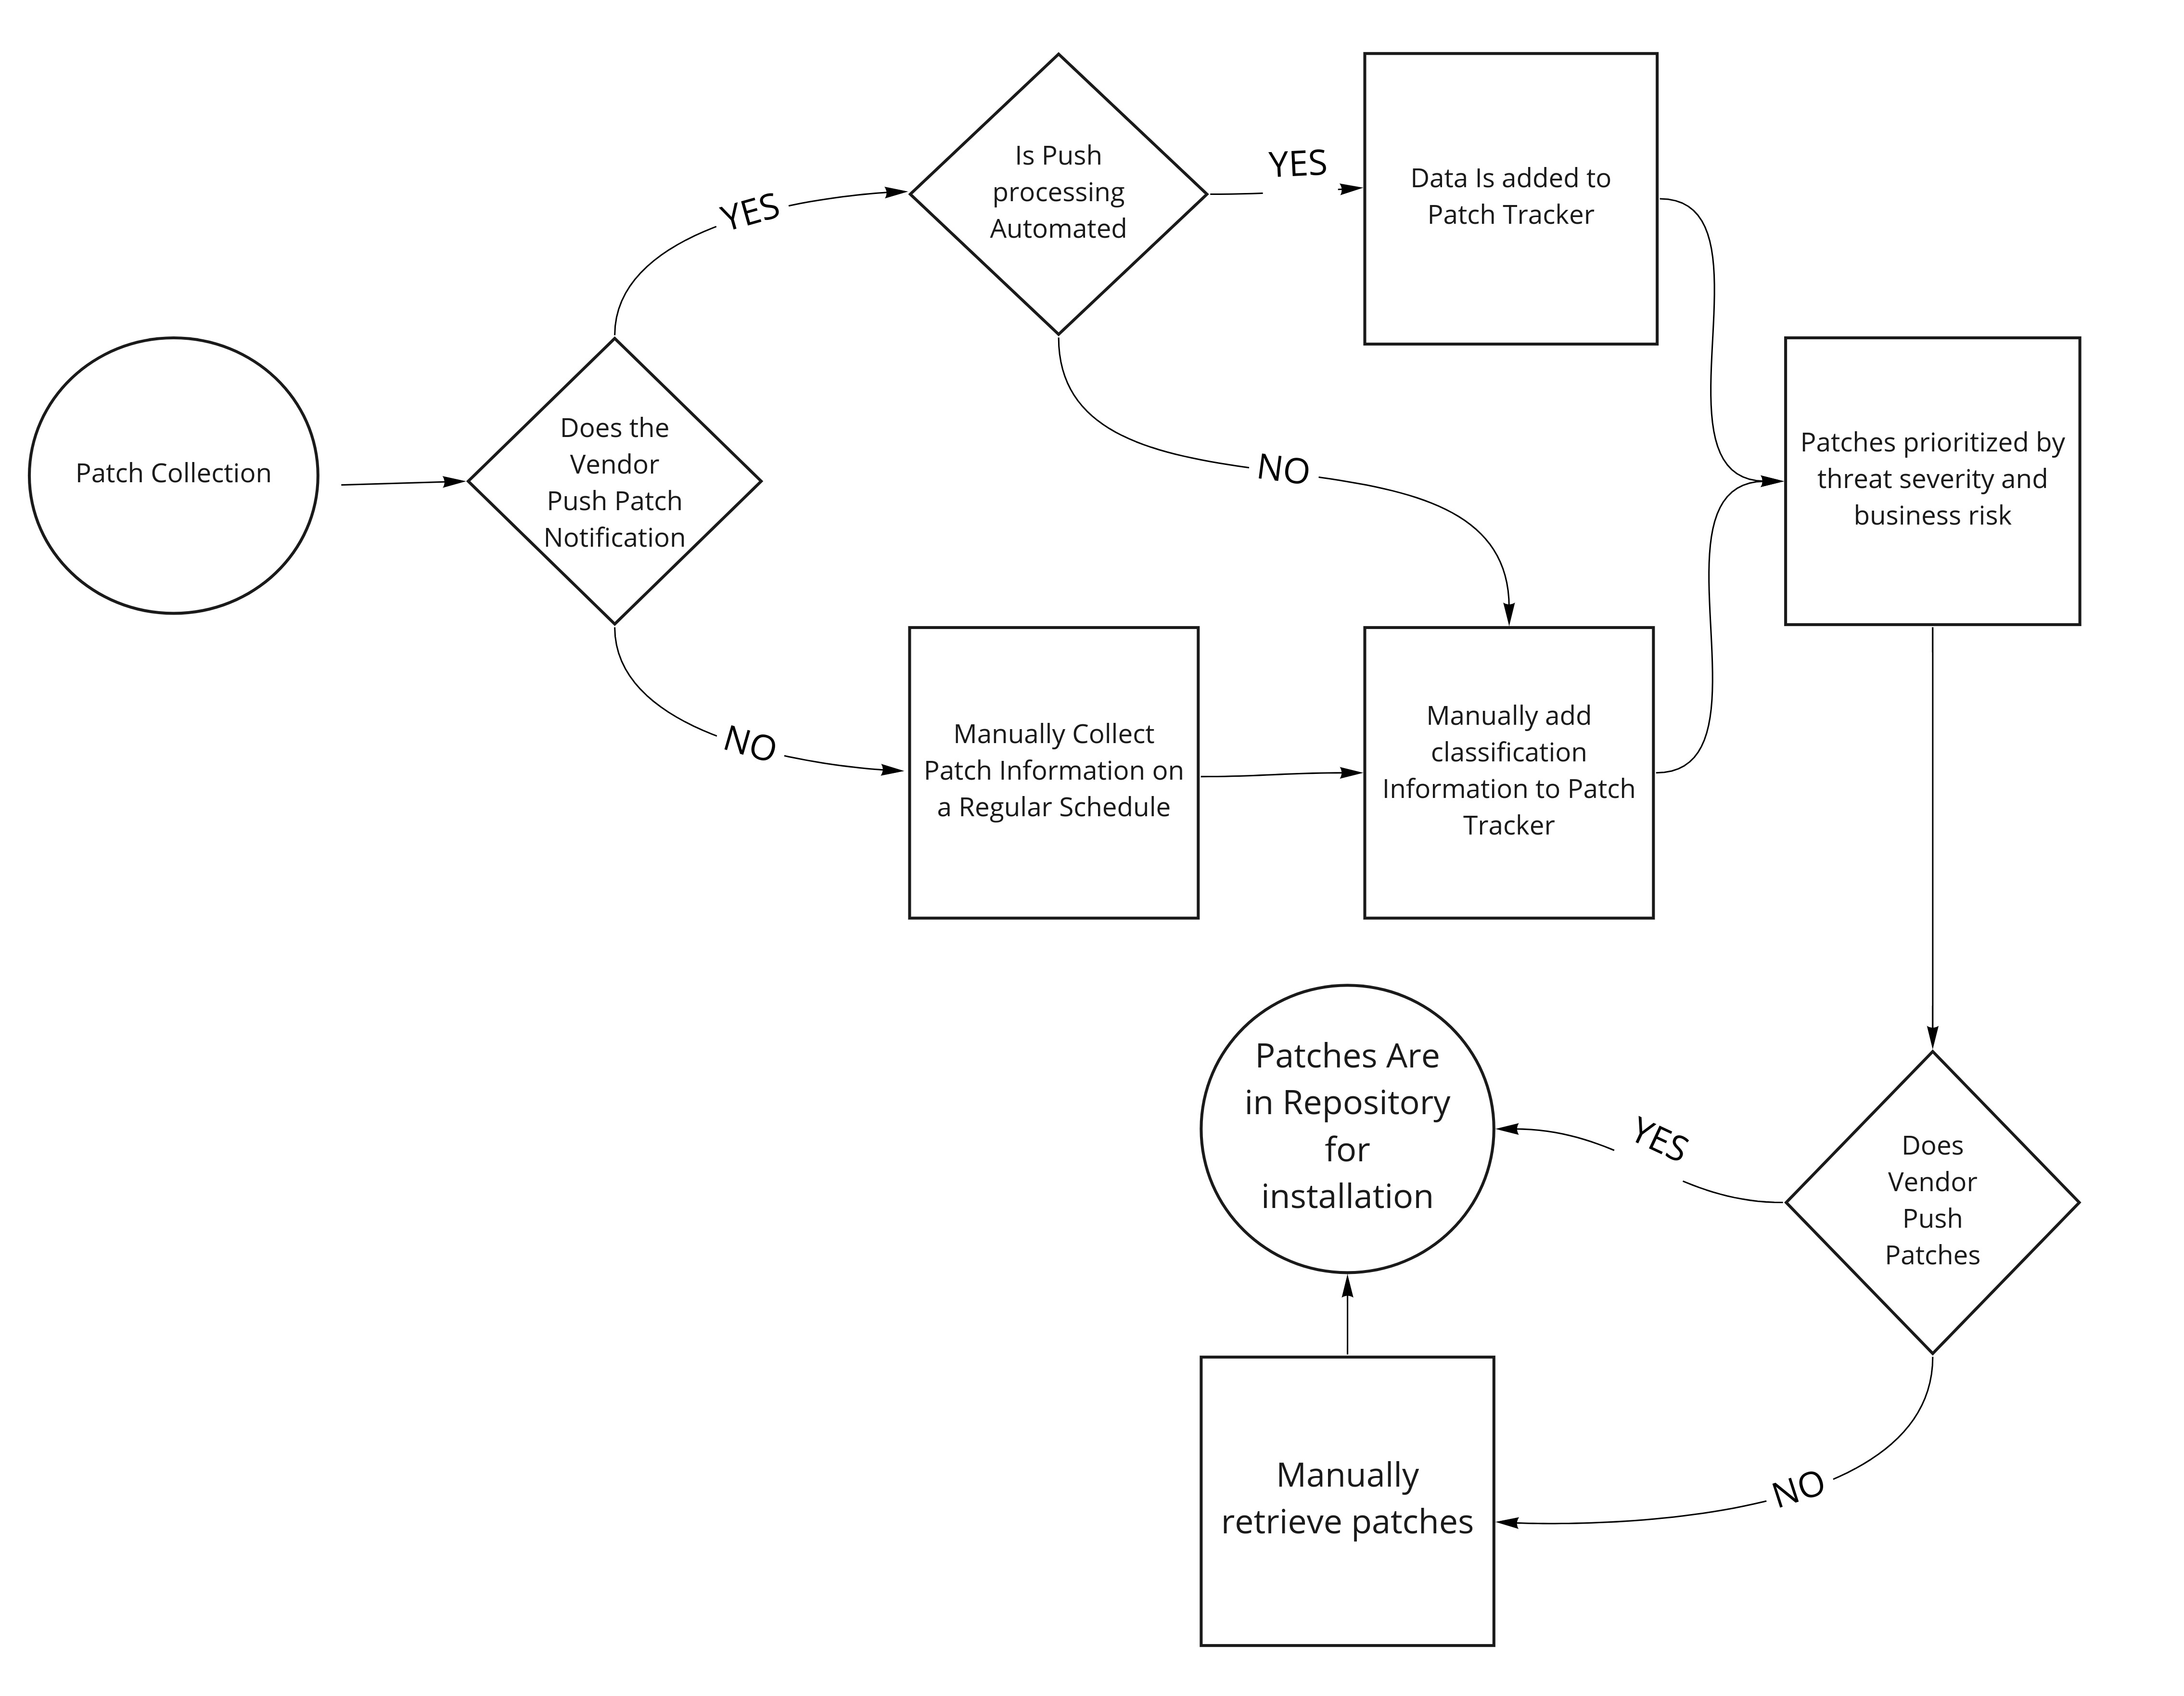
\includegraphics[width=0.8\textwidth]{img/collection}
\end{figure}

\note[item]{\scriptsize{Patch collection is the first portion of the patching process, and it is in many ways the most complex aspect of the activity, and is ripe for BPR attention. The first thing to note is that there is no standard way for vendors to release patch information. Some vendors provide email notifications; others simply put up information on their website; some do both; and lastly some, but not all, release patching information to central internet security information sites. }}

\note[item]{\scriptsize{For each product, the patch information must be collected. Once collected, the patch information must be analyzed to determine which products in the environment the patch relates to, the severity of the patch, and other critical information. Some patches, for example, should only be applied if particular features of a product are used, which may apply to some devices, but not others in the same company's environment.}}

\note[item]{\scriptsize{The patches must then be prioritized based on the combined information of the threat severity and the business risk involved in both patching and not patching particular devices. At this point, the patch itself must be collected and placed in the company's deployment pipeline for each of the particular devices in question. }}

\end{frame}
